\documentclass[12pt]{article}
\usepackage[margin=1in]{geometry}
\usepackage{amsmath,amssymb,booktabs,threeparttable,graphicx,float,natbib,setspace,hyperref}
\newcommand{\sym}[1]{\ensuremath{^{#1}}}
\onehalfspacing
\title{Growth for Whom? Airport Connectivity and the Distribution of National Income}
\author{Sunbin Yoo \and [coauthors]}
\date{Draft v2, 18 September 2026}

\begin{document}
\maketitle

\begin{abstract}
Gateway airports are associated with national income growth, but the distribution of that growth within countries has not been established. We combine the Global Airport Connectivity Index (GACI) for 1996--2023 with market and disposable income Gini coefficients from the Standardized World Income Inequality Database and pretax income shares from the World Inequality Database for 166 economies. Within-country increases in the connectivity of a country's primary hub are associated with a higher market-income Gini coefficient. The association is present in OLS with country and year fixed effects and larger in two-stage least squares that instrument connectivity with a Feyrer-type interaction between a global aviation-intensity index and baseline geographic air market access, and with a tourism-heritage instrument; the two instruments give statistically indistinguishable estimates. The market-Gini association is robust to continent by year fixed effects, to controls for baseline exposures interacted with the aviation index, and to income and inequality tercile by year fixed effects, whereas the disposable-income association is not robust to continent by year fixed effects. The response is located in the lower half of the distribution: the pretax income share of the bottom half falls, the top decile share rises by less, and the top percentile share does not respond. Connectivity raises GDP per capita, industrial employment and urbanisation, each of which is associated with lower inequality, so the residual association exceeds the total. Measured in income levels rather than shares, the same movement raises the average income of the top decile by about three times that of the bottom half, and the level estimates, unlike the ratio between the two, survive neither continent by year fixed effects nor the second instrument. Holding total national connectivity fixed, a more concentrated airport network is associated with higher inequality. Long-difference and Open Skies liberalisation designs do not move connectivity, so the evidence identifies within-country co-movement rather than the response to a discrete shock. The association is strongest in Asia and in the period after 2010.
\end{abstract}

\section{Introduction}
\label{sec:intro}
Whether air connectivity raises national income has been established in the accessibility literature; whether the resulting income is shared has not. Recent global evidence links the connectivity of a country's most connected airport to GDP per capita, inbound tourism and service exports, with the largest GDP association in the lowest development quartile \citep{Yue_2026}. National aggregates cannot show who receives these gains. A gateway hub concentrates high-skill business services, tourism employment and land rents in one metropolitan area, while the traffic it carries originates throughout the country. The distributional consequences of this concentration are the subject of this paper.

We ask whether hub connectivity makes national income more unequal. Connectivity is measured with the Global Airport Connectivity Index (GACI), which combines degree, eigenvector, closeness and flow-betweenness centrality with regional importance for 5,428 airports over 1996--2024 \citep{Cheung_2020}. Inequality is measured with the market and disposable income Gini coefficients of the Standardized World Income Inequality Database (SWIID) and with the pretax and post-tax income shares of the World Inequality Database (WID). The estimation sample covers 166 economies and 3,735 country-years.

Three features of the design are central. First, market and disposable inequality are treated separately, so that the response can be decomposed into a market component and a redistribution component. Second, the Gini is complemented with the income shares of the bottom half, the top decile and the top percentile, so that the location of the response along the distribution is observed rather than inferred. Third, two instruments that exploit different sources of variation are used, a Feyrer-type interaction between a global aviation-intensity index and each country's baseline geographic air market access \citep{Feyrer_2019} and a tourism-heritage interaction between world tourist arrivals and a country's fixed endowment of natural World Heritage sites. Because both instruments share the shift-share structure, whose validity depends on baseline exposures being unrelated to differential inequality trends, an extensive set of exposure-trend diagnostics is reported.

The paper makes three contributions. First, it provides the first global panel estimates of the association between airport connectivity and the within-country distribution of income. Second, it locates the response along the distribution and separates the market response from redistribution. Third, it shows that the composition of a national airport network is associated with the distribution of income conditional on the total amount of connectivity, which bears on the policy choice between hub concentration and distributed airport investment.

\section{Hypothesis development}
\label{sec:framework}
Four channels connect the connectivity of a national gateway to the distribution of income, and they do not all operate in the same direction, which is why the question is empirical.

The first channel is skill-biased demand. Hub connectivity lowers the cost of face-to-face interaction and therefore raises the demand for tradable business services, finance and professional occupations, which are concentrated among high earners \citep{Allen_2014,Brueckner_2003}. If this channel dominates, the top of the distribution gains. The second channel is tourism employment. Connectivity raises inbound tourism, whose direct employment is concentrated in accommodation and food services and is low-wage \citep{Khadaroo_2008}. If this channel dominates, the bottom of the distribution gains and inequality falls. The third channel is spatial concentration. A gateway city captures the location rents and agglomeration gains of connectivity, while the rest of the country supplies migrants and demand; the resulting interregional gap appears in national personal inequality \citep{Redding_2004}. The fourth channel is redistribution. Market inequality may rise while disposable inequality rises by less if governments redistribute part of the gains.

\begin{quote}
\textbf{Hypothesis 1 (Distribution).} Higher hub connectivity increases the market-income Gini coefficient. The disposable-income response is smaller than the market-income response.
\end{quote}
\begin{quote}
\textbf{Hypothesis 2 (Location).} The response is located at the tails: the pretax income share of the top decile rises and the share of the bottom half falls.
\end{quote}
\begin{quote}
\textbf{Hypothesis 3 (Concentration).} Conditional on total national connectivity, a network in which connectivity is concentrated in a single gateway is associated with higher inequality than a distributed network.
\end{quote}
\begin{quote}
\textbf{Hypothesis 4 (Mechanisms).} The association operates net of the income growth, structural transformation and urbanisation that connectivity induces; these induced changes are themselves associated with lower inequality, so that the residual association exceeds the total.
\end{quote}

\section{Data}
\label{sec:data}
The panel combines the airport-year GACI data of the companion papers with three inequality sources. Connectivity is aggregated to the country-year in three ways: the maximum across the country's airports (hub connectivity, $\mathrm{GACI}_{max}$), the seat-capacity-weighted mean (hub quality, $\mathrm{GACI}_{cwm}$) and the sum across airports (total connectivity, $\mathrm{GACI}_{sum}$). Two concentration measures summarise the composition of the network: the share of the top airport in the national sum and the Herfindahl index of airport shares.

Inequality is measured in three ways. The SWIID (version 9) provides market-income and disposable-income Gini coefficients for 199 economies with model-based standard errors; we use the point estimates and report country-clustered inference throughout \citep{Solt_2020}. The WID provides pretax and post-tax national income shares for the bottom 50 percent, the middle 40 percent, the top 10 percent and the top 1 percent of equal-split adults, together with a Gini derived from the same distributions \citep{WID_2024}. The World Bank Poverty and Inequality Platform provides survey-based Gini coefficients and decile shares for survey years only and serves as an independent check. Controls and mechanism variables (population, GDP per capita, sectoral employment shares, urbanisation, urban primacy, unemployment, trade, FDI, tax revenue and tertiary enrolment) come from the World Development Indicators.

The estimation sample is the intersection of the connectivity panel with the SWIID: 166 economies and 3,735 country-years over 1996--2023. Table~\ref{tab:sumstat} reports summary statistics. Two features of the data matter for what follows. First, inequality is slow moving: the within-country standard deviation of the market Gini is 1.7 points against a cross-sectional standard deviation of 6.4. Second, hub connectivity also varies mainly across countries: the within standard deviation of $\ln\mathrm{GACI}_{max}$ is 0.16 against 0.61 overall. Both features limit the information available in short differences, to which we return in Section~\ref{sec:horizon}.

\begin{table}[H]\centering\caption{Summary statistics, estimation sample (166 economies, 1996--2023).}\label{tab:sumstat}
\begin{threeparttable}\small\begin{tabular}{lrrrrrr}
\toprule
Variable & N & Mean & SD & Within SD & Min & Max \\
\midrule
Market-income Gini (SWIID) & 3,737 & 45.594 & 6.413 & 1.672 & 31.200 & 72.400 \\
Disposable-income Gini (SWIID) & 3,737 & 38.363 & 8.193 & 1.678 & 22.100 & 65.800 \\
Top 10\% pretax income share (WID) & 3,716 & 0.453 & 0.093 & 0.025 & 0.255 & 0.687 \\
Bottom 50\% pretax income share (WID) & 3,716 & 0.150 & 0.047 & 0.012 & 0.051 & 0.279 \\
Hub connectivity, GACI max & 3,737 & 1.319 & 0.612 & 0.157 & 0.534 & 3.626 \\
Hub quality, GACI cwm & 3,737 & 1.124 & 0.416 & 0.115 & 0.534 & 3.014 \\
Total connectivity, GACI sum & 3,737 & 16.589 & 46.228 & 6.274 & 0.545 & 510.036 \\
Share of top airport in national GACI & 3,737 & 0.366 & 0.329 & 0.105 & 0.006 & 1.000 \\
Airports per country & 3,737 & 22.272 & 57.942 & 6.996 & 1.000 & 614.000 \\
Feyrer instrument & 3,737 & 4.606 & 4.227 & 4.104 & 0.000 & 14.667 \\
Tourism-heritage instrument & 3,737 & 0.475 & 0.478 & 0.276 & 0.000 & 2.944 \\
ln population & 3,737 & 16.095 & 1.805 & 0.125 & 9.778 & 21.078 \\
ln GDP per capita & 3,737 & 8.587 & 1.446 & 0.222 & 5.426 & 11.630 \\
\bottomrule
\end{tabular}
\begin{tablenotes}\footnotesize\item Within SD is the standard deviation after removing country means. Gini coefficients in points; income shares as fractions.\end{tablenotes}\end{threeparttable}\end{table}

Figure~\ref{fig:map_base} maps hub connectivity in 2023. The gateway economies of North America, Western Europe, the Gulf and East Asia occupy the top of the distribution and most of sub-Saharan Africa and Central Asia the bottom; the cross-sectional range of $\ln\mathrm{GACI}_{max}$ is $-0.55$ to $1.18$ against a within-country standard deviation of $0.16$.

\begin{figure}[H]\centering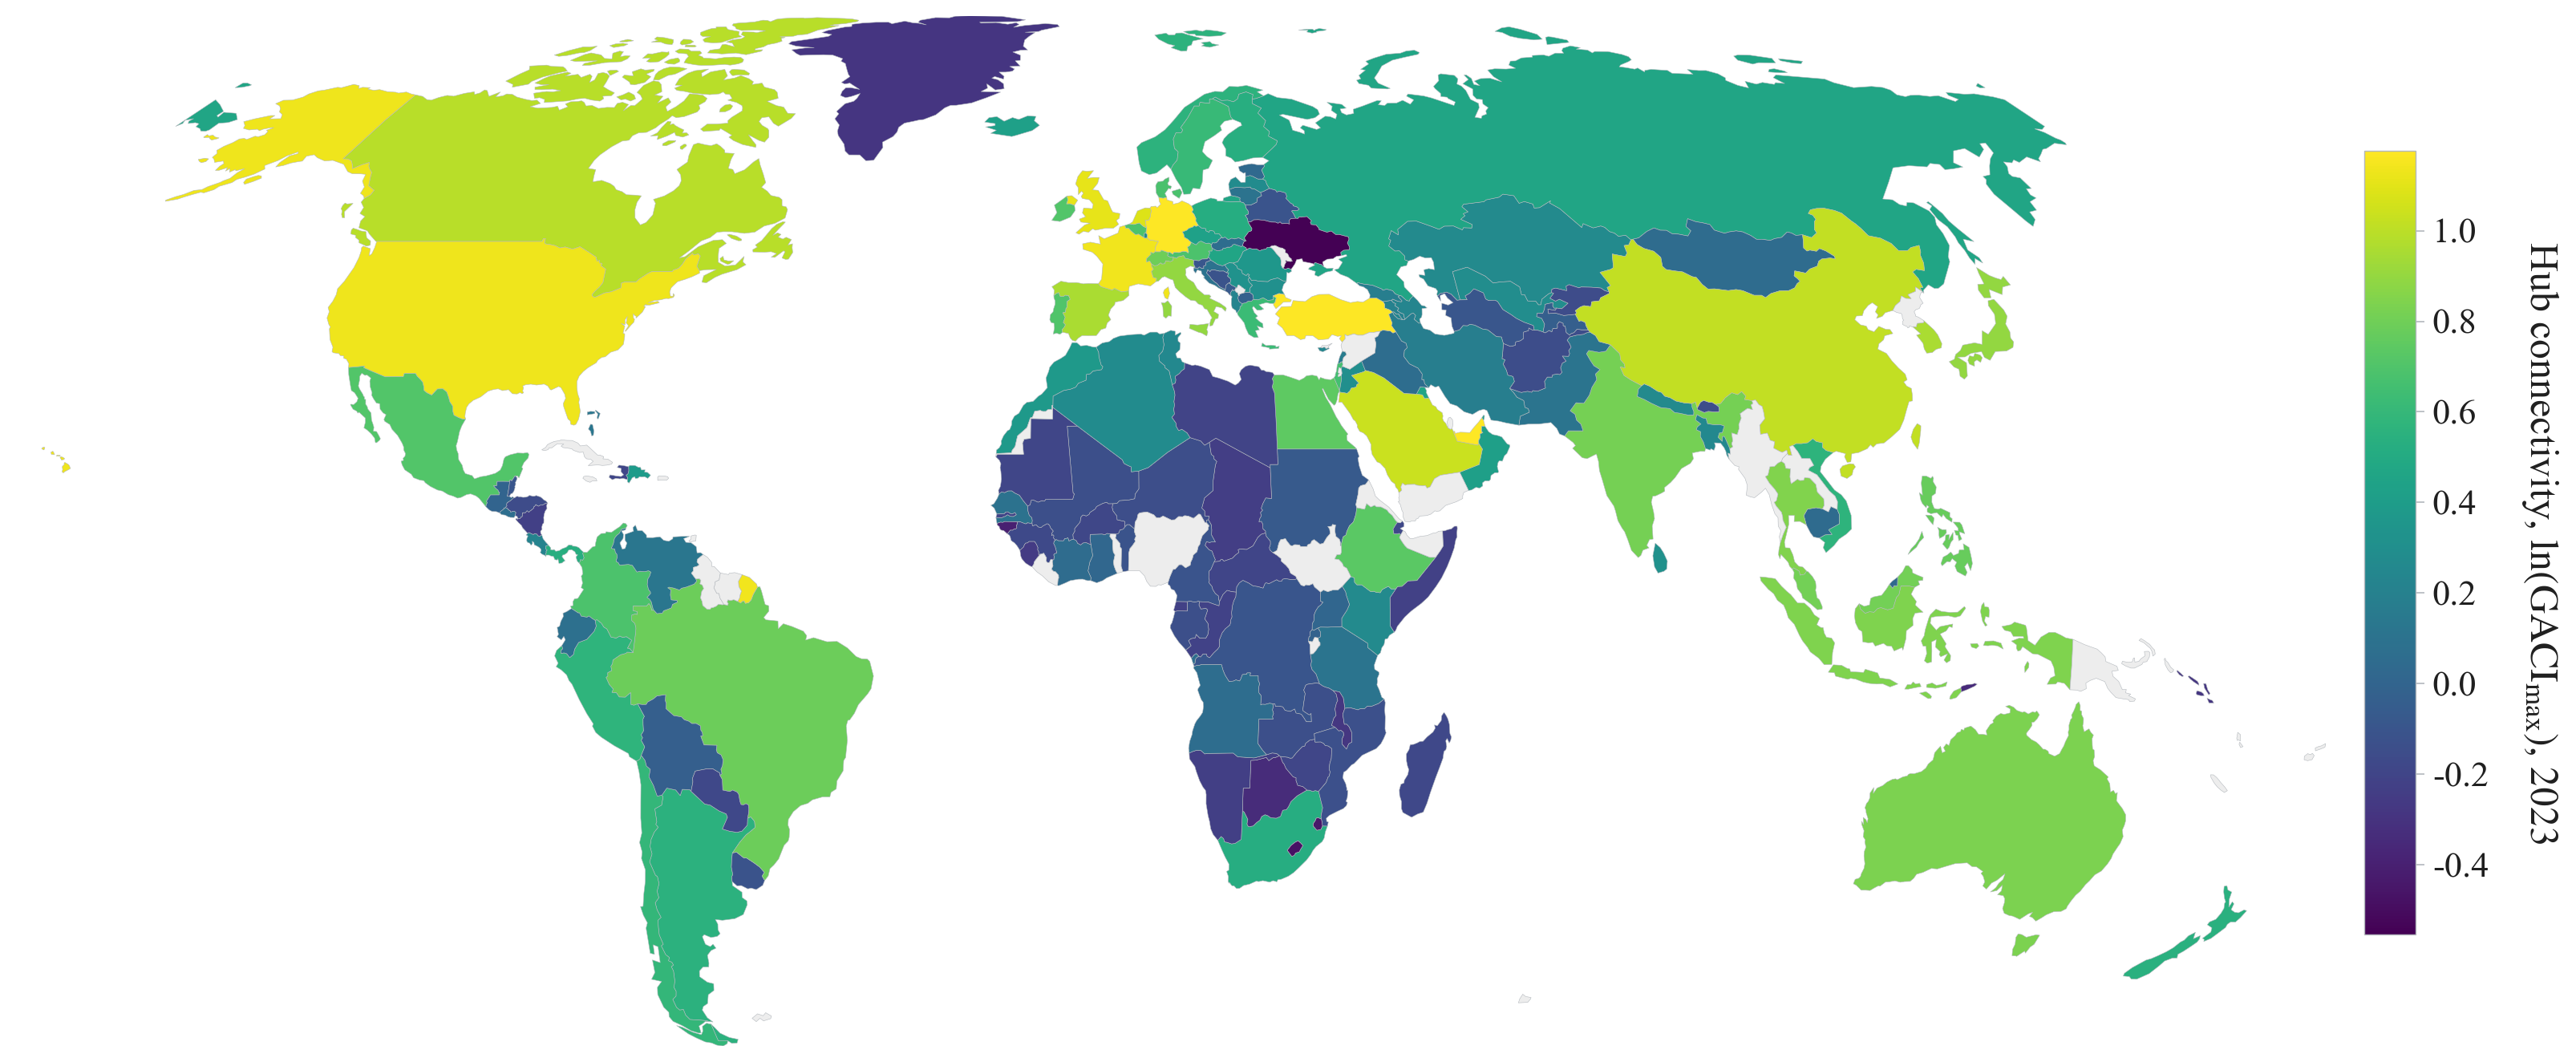
\includegraphics[width=\linewidth]{fig_map_base_gacimax.png}
\caption{Hub connectivity, $\ln\mathrm{GACI}_{max}$, 2023. Grey denotes economies outside the estimation sample.}\label{fig:map_base}\end{figure}

\section{Empirical strategy}
\label{sec:strategy}
The baseline specification relates within-country changes in inequality to within-country changes in connectivity:
\begin{equation}
\ln G_{ct} = \beta \ln \mathrm{GACI}_{ct} + \gamma \ln \mathrm{Pop}_{ct} + \mu_c + \lambda_t + \varepsilon_{ct},
\label{eq:base}
\end{equation}
where $G_{ct}$ is the Gini coefficient or an income share of country $c$ in year $t$, and $\mu_c$ and $\lambda_t$ are country and year fixed effects. Following the companion papers, the baseline controls only for population; GDP per capita, trade and the sectoral structure are outcomes of connectivity and enter as candidate mechanisms rather than as controls. Standard errors are heteroskedasticity-robust in the main tables, with country-clustered standard errors reported in brackets and used for the two-stage least squares (2SLS) inference in the text.

Connectivity is not assigned at random. Route development follows expected demand, and the policy reforms that attract airlines may also change the distribution of income. We therefore instrument $\ln\mathrm{GACI}_{ct}$ with the Feyrer interaction $Z^{F}_{ct} = a_t \times \ln\mathrm{MA}^{air}_{c,1996}$, where $a_t$ is a global aviation-intensity index normalised to $[0,1]$ and $\mathrm{MA}^{air}_{c,1996}$ is the population-weighted great-circle market access of the country's airports in the base year \citep{Feyrer_2019}. The identifying assumption is that, conditional on the fixed effects, countries whose geography placed them to benefit more from the global expansion of aviation did not experience differential inequality trends for other reasons. The tourism-heritage instrument $Z^{T}_{ct}$ interacts world international tourist arrivals with the country's fixed endowment of natural and mixed World Heritage sites and identifies connectivity growth on the leisure margin. The two instruments differ in the exposure they use, so agreement between them is informative, and the Hansen $J$ test of over-identification is reported.

Both instruments are shift-share instruments with a single global shifter. Their validity therefore rests on the exposure variable, which we probe in four ways in Section~\ref{sec:diag}: continent by year fixed effects, controls for other baseline exposures (income, inequality, land area, latitude, sea market access) interacted with the same aviation index, income and inequality tercile by year fixed effects, and first stages estimated separately by continent.

\section{Main results}
\label{sec:results}
We begin by asking whether hub connectivity is associated with the level of inequality within countries. This is the first-order question for the distributional reading of connectivity: if the market Gini does not move with the primary hub, the channels in Section~\ref{sec:framework} cancel in the aggregate. Table~\ref{tab:main} reports, for each connectivity measure, the OLS estimate, the first stage of each instrument and the 2SLS estimates for the market and disposable Gini coefficients. All specifications include country and year fixed effects and log population; first-stage statistics are reported within the table.

Panel A uses hub connectivity, the headline measure. In OLS, a one-percent increase in hub connectivity is associated with a $0.061$ percent increase in the market Gini. The 2SLS estimate is $0.495$ with the Feyrer instrument and $0.468$ with the tourism instrument, and the two instruments therefore agree on sign and magnitude; the Hansen $J$ test does not reject their joint validity for the market Gini ($p=0.88$, Table~\ref{tab:robust}). For example, a coefficient of $0.495$ means that a 10 percent increase in hub connectivity is associated with a 5 percent increase in the market Gini, or about 2.3 points at the sample mean of 45.6. The disposable Gini responds by a similar amount in OLS ($0.050$) and by more in 2SLS ($0.651$ with the Feyrer instrument, $0.391$ with the tourism instrument). The first part of Hypothesis~1 is supported; the second part, that redistribution attenuates the response, is not, since the disposable response is not smaller than the market response.

Panel B uses hub quality and Panel C total connectivity. The pattern of signs and significance is unchanged. The sum measure has the smallest coefficients because it scales with the number of airports, and the capacity-weighted mean has the largest, consistent with connectivity concentrated at large airports being the relevant margin. The three measures are on different scales; what carries across them is the common pattern of a positive OLS estimate, a larger 2SLS estimate, and agreement between the two instruments. Table~\ref{tab:a_levels} reports the same specifications with the Gini in points, and Table~\ref{tab:a_absred} reports absolute redistribution as an outcome.

The 2SLS estimates are about eight times the OLS estimates. Three explanations are consistent with the data. First, measurement error in the aggregated index attenuates OLS. Second, the instruments identify the response of countries whose connectivity growth was driven by global aviation expansion and geography, which may be the countries in which connectivity growth was least accompanied by compensating policy. Third, the instruments may partly capture differential trends, which Section~\ref{sec:diag} examines. We report both estimates throughout and treat the OLS estimate as a lower bound and the 2SLS estimate as an upper bound when quantifying the association.

\begin{table}[H]\centering\caption{Main results: OLS, first stage, and 2SLS, by connectivity measure.}\label{tab:main}
\begin{threeparttable}\small\begin{tabular}{lcc}
\toprule
 & Market-income Gini & Disposable-income Gini \\
 & $\ln G^{mkt}$ & $\ln G^{disp}$ \\
\midrule
\multicolumn{3}{l}{\emph{Panel A. Hub connectivity, $\ln\mathrm{GACI}_{max}$ (headline)}}\\
First stage, Feyrer instrument & \multicolumn{2}{l}{0.146\sym{***}\ \ (0.015),\ \ KP $F=98.5$} \\
First stage, Tourism-heritage instrument & \multicolumn{2}{l}{0.038\sym{***}\ \ (0.010),\ \ KP $F=13.6$} \\
OLS & 0.061\sym{***} (0.008) & 0.050\sym{***} (0.009) \\
2SLS, Feyrer IV & 0.495\sym{***} (0.062) & 0.651\sym{***} (0.077) \\
 & [0.194]\sym{**} & [0.241]\sym{***} \\
2SLS, tourism IV & 0.468\sym{***} (0.165) & 0.391\sym{***} (0.151) \\
 & [0.260]\sym{*} & [0.284] \\
\addlinespace
\multicolumn{3}{l}{\emph{Panel B. Hub quality, $\ln\mathrm{GACI}_{cwm}$}}\\
First stage, Feyrer instrument & \multicolumn{2}{l}{0.122\sym{***}\ \ (0.013),\ \ KP $F=83.2$} \\
First stage, Tourism-heritage instrument & \multicolumn{2}{l}{0.024\sym{***}\ \ (0.009),\ \ KP $F=6.9$} \\
OLS & 0.079\sym{***} (0.009) & 0.060\sym{***} (0.010) \\
2SLS, Feyrer IV & 0.595\sym{***} (0.076) & 0.783\sym{***} (0.096) \\
 & [0.240]\sym{**} & [0.302]\sym{***} \\
2SLS, tourism IV & 0.726\sym{**} (0.313) & 0.607\sym{**} (0.283) \\
 & [0.547] & [0.530] \\
\addlinespace
\multicolumn{3}{l}{\emph{Panel C. Total connectivity, $\ln\mathrm{GACI}_{sum}$}}\\
First stage, Feyrer instrument & \multicolumn{2}{l}{0.364\sym{***}\ \ (0.034),\ \ KP $F=113.4$} \\
First stage, Tourism-heritage instrument & \multicolumn{2}{l}{0.068\sym{***}\ \ (0.023),\ \ KP $F=9.0$} \\
OLS & 0.008\sym{***} (0.002) & 0.009\sym{***} (0.003) \\
2SLS, Feyrer IV & 0.199\sym{***} (0.026) & 0.262\sym{***} (0.031) \\
 & [0.077]\sym{***} & [0.090]\sym{***} \\
2SLS, tourism IV & 0.260\sym{***} (0.099) & 0.217\sym{**} (0.093) \\
 & [0.191] & [0.187] \\
\addlinespace
\midrule
Country, Year FE & Yes & Yes \\
Observations & 3,735 & 3,735 \\
\bottomrule
\end{tabular}
\begin{tablenotes}\footnotesize\item Robust SE in parentheses; country-clustered SE in brackets with the corresponding significance level. The first-stage rows regress the connectivity measure on the instrument with population and two-way fixed effects; KP $F$ is the Kleibergen--Paap statistic with robust errors. \sym{*}~$p<0.10$, \sym{**}~$p<0.05$, \sym{***}~$p<0.01$.\end{tablenotes}\end{threeparttable}\end{table}

\subsection{Growth and its incidence}
\label{sec:growth}
Does hub connectivity also move average income, and if so, who receives the increase? This matters for reading Table~\ref{tab:main}: a rising Gini that accompanies broad income growth is a different object from a rising Gini in which the bottom half stands still. Table~\ref{tab:growth} reports the specifications of Table~\ref{tab:main} with growth outcomes, and Table~\ref{tab:growth_decomp} separates the response of each group's average income into a level term that both groups share and a share term that they do not.

Average income moves with connectivity, and by more than any distribution estimate in this paper. In OLS a one-percent increase in hub connectivity accompanies a $0.75$ percent increase in GDP per capita, and in 2SLS with the Feyrer instrument the elasticity is $1.29$. The World Inequality Database measure of average pretax income per adult, which is built from national accounts rather than from the World Development Indicators, gives $0.67$ and $1.22$ in the same specifications, so the two income sources agree on the sign and on the order of magnitude.

The increase is not shared evenly. Under the Feyrer instrument the average income of the top decile rises by $1.44$ percent per percent of connectivity, the average income of the bottom half by $0.45$ percent, and the ratio between the two by $1.00$ percent. Table~\ref{tab:growth_decomp} shows where the difference arises. Both groups carry the same level term of $1.22$. The top decile adds a share gain of $0.22$ and the bottom half subtracts a share loss of $0.77$, which is the estimate already reported in Table~\ref{tab:tails}. The bottom half therefore retains about one third of the average gain. Consider an economy whose hub connectivity rises by ten percent. Average income rises by about twelve percent, the average income of the top decile by about fourteen percent and that of the bottom half by about four percent, while the market Gini rises by about five percent of its own value, which is $2.3$ points at the sample mean of $45.6$. Growth and the rise in the Gini are two readings of one movement rather than two separate findings.

The growth estimates are less robust than the distribution estimates, and three results set the limit. First, the tourism-heritage instrument, which reproduces the market-Gini estimate of the Feyrer instrument ($0.47$ against $0.50$), gives $-0.13$ for GDP per capita and cannot be distinguished from zero; with both instruments entered together the Hansen test rejects for GDP per capita ($p=0.002$), for average income ($p<0.001$) and for the top decile ($p=0.004$), but not for the top-to-bottom ratio ($p=0.33$). Second, under continent by year fixed effects the level estimates turn negative, $-1.07$ for GDP per capita and $-1.68$ for the bottom half, while the ratio remains positive at $1.21$ and significant (Table~\ref{tab:a_growth_diag}). Third, in long differences the instrument is uninformative for growth as it is for inequality, with a first-stage $F$ below $3$ in every window (Table~\ref{tab:a_growth_ld}), and the leads are as large as the lags (Table~\ref{tab:a_growth_hzn}). What survives these checks is the incidence rather than the level, so we treat the level estimates as descriptive and the gap estimates as the result.

One feature of the construction separates the two halves of Table~\ref{tab:growth_decomp}. The Gini coefficients and the income shares are distribution statistics and do not use national income in their construction, so their co-movement with GDP per capita is an estimate rather than an identity. The group average incomes in the last three columns of Table~\ref{tab:growth} do share a national-accounts level term by construction, and that term is what row 1 of Table~\ref{tab:growth_decomp} isolates and the ratio removes.

\begin{table}[H]\centering\caption{Growth outcomes: GDP per capita and group average incomes.}\label{tab:growth}
\begin{threeparttable}\small\begin{tabular}{lccccc}
\toprule
 & GDP per capita & Average income & Top 10\% average & Bottom 50\% average & Top/bottom gap \\
 & $\ln y$ & $\ln \bar{y}$ & $\ln \bar{y}^{t10}$ & $\ln \bar{y}^{b50}$ & $\ln(\bar{y}^{t10}/\bar{y}^{b50})$ \\
\midrule
\multicolumn{6}{l}{\emph{Panel A. Hub connectivity, $\ln\mathrm{GACI}_{max}$ (headline)}}\\
OLS & 0.747\sym{***} (0.042) & 0.668\sym{***} (0.043) & 0.747\sym{***} (0.042) & 0.586\sym{***} (0.051) & 0.161\sym{***} (0.034) \\
2SLS, Feyrer IV & 1.294\sym{***} (0.152) & 1.219\sym{***} (0.173) & 1.443\sym{***} (0.184) & 0.445\sym{**} (0.200) & 0.998\sym{***} (0.189) \\
 & [0.428]\sym{***} & [0.491]\sym{**} & [0.513]\sym{***} & [0.593] & [0.588]\sym{*} \\
2SLS, tourism IV & -0.133 (0.559) & -0.394 (0.573) & -0.013 (0.557) & -0.506 (0.622) & 0.493 (0.414) \\
 & [1.127] & [1.142] & [1.120] & [1.268] & [0.975] \\
First-stage KP $F$ (Feyrer; tourism) & 98; 14 & 97; 13 & 97; 13 & 97; 13 & 97; 13 \\
\addlinespace
\multicolumn{6}{l}{\emph{Panel B. Hub quality, $\ln\mathrm{GACI}_{cwm}$}}\\
OLS & 0.775\sym{***} (0.043) & 0.708\sym{***} (0.044) & 0.774\sym{***} (0.046) & 0.656\sym{***} (0.050) & 0.118\sym{***} (0.037) \\
2SLS, Feyrer IV & 1.556\sym{***} (0.194) & 1.462\sym{***} (0.214) & 1.731\sym{***} (0.229) & 0.533\sym{**} (0.241) & 1.197\sym{***} (0.231) \\
 & [0.548]\sym{***} & [0.611]\sym{**} & [0.633]\sym{***} & [0.715] & [0.709]\sym{*} \\
2SLS, tourism IV & -0.206 (0.882) & -0.612 (0.932) & -0.019 (0.866) & -0.785 (1.025) & 0.766 (0.682) \\
 & [1.748] & [1.791] & [1.738] & [2.027] & [1.603] \\
First-stage KP $F$ (Feyrer; tourism) & 83; 7 & 83; 7 & 83; 7 & 83; 7 & 83; 7 \\
\addlinespace
\multicolumn{6}{l}{\emph{Panel C. Total connectivity, $\ln\mathrm{GACI}_{sum}$}}\\
OLS & 0.185\sym{***} (0.012) & 0.172\sym{***} (0.012) & 0.178\sym{***} (0.013) & 0.166\sym{***} (0.013) & 0.013 (0.010) \\
2SLS, Feyrer IV & 0.520\sym{***} (0.067) & 0.497\sym{***} (0.076) & 0.589\sym{***} (0.082) & 0.181\sym{**} (0.084) & 0.407\sym{***} (0.075) \\
 & [0.173]\sym{***} & [0.200]\sym{**} & [0.213]\sym{***} & [0.246] & [0.233]\sym{*} \\
2SLS, tourism IV & -0.074 (0.312) & -0.223 (0.331) & -0.007 (0.315) & -0.286 (0.360) & 0.279 (0.238) \\
 & [0.628] & [0.657] & [0.633] & [0.749] & [0.597] \\
First-stage KP $F$ (Feyrer; tourism) & 113; 9 & 109; 9 & 109; 9 & 109; 9 & 109; 9 \\
\addlinespace
\multicolumn{6}{l}{\emph{Panel D. Both instruments, $\ln\mathrm{GACI}_{max}$ (over-identified)}}\\
2SLS, Feyrer and tourism & 1.045\sym{***} (0.133) & 0.937\sym{***} (0.150) & 1.188\sym{***} (0.163) & 0.279 (0.175) & 0.910\sym{***} (0.157) \\
Hansen $J$ ($p$) & 0.002 & 0.000 & 0.004 & 0.090 & 0.328 \\
\midrule
Country, Year FE & Yes & Yes & Yes & Yes & Yes \\
Observations & 3,735 & 3,714 & 3,714 & 3,714 & 3,714 \\
\bottomrule
\end{tabular}
\begin{tablenotes}\footnotesize\item GDP per capita is World Development Indicators output in constant 2015 US dollars. Average incomes are World Inequality Database pretax national income per equal-split adult aged 20 and over, in constant local currency, so country fixed effects absorb the currency unit. Robust SE in parentheses, country-clustered SE in brackets with the corresponding significance level. Log population and country and year fixed effects throughout. Panel D enters both instruments; the Hansen row reports the over-identification test. \sym{*}~$p<0.10$, \sym{**}~$p<0.05$, \sym{***}~$p<0.01$.\end{tablenotes}\end{threeparttable}\end{table}

\begin{table}[H]\centering\caption{Incidence of the income gain: level and share components (hub connectivity).}\label{tab:growth_decomp}
\begin{threeparttable}\small\begin{tabular}{lccc}
\toprule
 & Top 10\% & Bottom 50\% & Gap \\
\midrule
\multicolumn{4}{l}{\emph{Panel A. OLS}}\\
(1) Average income, all adults & 0.668\sym{***} (0.043) & 0.668\sym{***} (0.043) & -- \\
(2) Group income share & 0.079\sym{***} (0.015) & -0.082\sym{***} (0.020) & 0.161\sym{***} (0.034) \\
(3) Group average income $=(1)+(2)$ & 0.747\sym{***} (0.042) & 0.586\sym{***} (0.051) & 0.161\sym{***} (0.034) \\
Memo: market-income Gini & \multicolumn{3}{c}{0.061\sym{***} (0.008)} \\
\addlinespace
\multicolumn{4}{l}{\emph{Panel B. 2SLS, Feyrer instrument}}\\
(1) Average income, all adults & 1.219\sym{***} (0.173) & 1.219\sym{***} (0.173) & -- \\
(2) Group income share & 0.224\sym{***} (0.063) & -0.774\sym{***} (0.134) & 0.998\sym{***} (0.189) \\
(3) Group average income $=(1)+(2)$ & 1.443\sym{***} (0.184) & 0.445\sym{**} (0.200) & 0.998\sym{***} (0.189) \\
Memo: market-income Gini & \multicolumn{3}{c}{0.495\sym{***} (0.062)} \\
\addlinespace
\midrule
Country, Year FE & Yes & Yes & Yes \\
Observations & 3,714 & 3,714 & 3,714 \\
\bottomrule
\end{tabular}
\begin{tablenotes}\footnotesize\item The rows are an accounting identity: the log average income of a group equals the log average income of all adults plus the log of the group's income share, up to a group-specific constant that the fixed effects absorb. Row 1 is therefore common to both columns and row 2 carries the distribution. Row 2 repeats the share estimates of Table~\ref{tab:tails}. The Gini and the income shares do not use national income in their construction; the group average incomes do. \sym{*}~$p<0.10$, \sym{**}~$p<0.05$, \sym{***}~$p<0.01$.\end{tablenotes}\end{threeparttable}\end{table}

\subsection{Heterogeneity by development, initial inequality and period}
\label{sec:hetero}
We next ask whether the association differs with the level of development, the initial level of inequality and the period. This matters for interpretation: if the association is confined to high-income or already-unequal economies, it reflects a different set of channels than if it is general. Table~\ref{tab:hetero} reports interaction 2SLS estimates in which both the connectivity measure and the instrument are interacted with fixed baseline group indicators, together with separate 2SLS by continent.

Panel A shows that the response is not monotone in development. The estimate is $0.47$ in the low-income tercile, $0.20$ in the middle tercile and $0.51$ in the high-income tercile, and the middle-tercile interaction is negative and significant. Separate regressions by tercile show that the low-income first stage is weak, so the U-shape rests mainly on the contrast between middle and high income (Table~\ref{tab:a_inc3split}). Panel B shows that the response is largest where inequality was initially low or moderate: $0.43$ in the lowest baseline-Gini tercile, $0.52$ in the middle and $0.33$ in the highest. Panel C shows that the response is larger after 2010 by $0.08$, the period in which low-cost and Gulf-carrier network expansion was concentrated.

Panel D reports the continent-specific estimates. The positive association is concentrated in Asia ($0.48$). The African estimate is negative ($-0.21$), the European and Latin American estimates are close to zero, and the Middle East, North America and Oceania estimates are imprecise, each resting on a first stage with $F$ below $2$. The African sign reversal is consistent with aviation substituting for missing surface transport in the least connected economies, where the first scheduled connections raise incomes in peripheral areas. The continent estimates also show that the first stage changes sign across continents (Table~\ref{tab:diag}), which Section~\ref{sec:diag} discusses. Overall, the association is general across income and inequality groups but is carried by Asia and by the period after 2010.

\begin{table}[H]\centering\caption{Heterogeneity: interaction 2SLS with the Feyrer instrument (robust SE).}\label{tab:hetero}
\begin{threeparttable}\small\begin{tabular}{lcc}
\toprule
 & $\ln G^{mkt}$ & $\ln G^{disp}$ \\
\midrule
\multicolumn{3}{l}{\emph{Panel A. Baseline GDP per capita tercile (interaction IV)}}\\
Low tercile (base) & 0.473\sym{***} (0.071) & 0.717\sym{***} (0.089) \\
Middle tercile (total) & 0.200\sym{***} (0.053) & 0.356\sym{***} (0.065) \\
High tercile (total) & 0.511\sym{***} (0.051) & 0.610\sym{***} (0.062) \\
Interaction: middle & -0.273\sym{***} (0.041) & -0.361\sym{***} (0.054) \\
Interaction: high & 0.038 (0.044) & -0.107\sym{*} (0.057) \\
\addlinespace\multicolumn{3}{l}{\emph{Panel B. Baseline market-Gini tercile (interaction IV)}}\\
Low tercile (base) & 0.425\sym{***} (0.054) & 0.543\sym{***} (0.067) \\
Middle tercile (total) & 0.515\sym{***} (0.069) & 0.714\sym{***} (0.088) \\
High tercile (total) & 0.331\sym{***} (0.070) & 0.437\sym{***} (0.089) \\
Interaction: middle & 0.090\sym{**} (0.038) & 0.171\sym{***} (0.049) \\
Interaction: high & -0.094\sym{**} (0.037) & -0.107\sym{**} (0.047) \\
\addlinespace\multicolumn{3}{l}{\emph{Panel C. Temporal: post-2010 interaction}}\\
Pre-2010 (base) & 0.401\sym{***} (0.069) & 0.521\sym{***} (0.088) \\
Post-2010 (total) & 0.479\sym{***} (0.060) & 0.628\sym{***} (0.077) \\
Interaction: post-2010 & 0.078\sym{**} (0.034) & 0.107\sym{**} (0.044) \\
\addlinespace\multicolumn{3}{l}{\emph{Panel D. By continent (separate 2SLS; KP $F$ in brackets)}}\\
Africa & -0.211\sym{***} (0.072) [40.6] & -0.146\sym{**} (0.070) [40.6] \\
Asia & 0.479\sym{***} (0.095) [27.2] & 0.365\sym{***} (0.094) [27.2] \\
Europe & -0.094 (0.068) [43.5] & -0.328\sym{***} (0.079) [43.5] \\
Latin America & -0.079 (0.294) [5.5] & -0.515 (0.340) [5.5] \\
Middle East & 0.739 (0.815) [1.1] & 0.402 (0.544) [1.1] \\
North America & -0.809 (0.682) [1.1] & -1.130 (1.043) [1.1] \\
Oceania & 3.350 (37.154) [0.0] & 3.565 (39.845) [0.0] \\
\bottomrule
\end{tabular}
\begin{tablenotes}\footnotesize\item Terciles are fixed at each country's first observed year. Total rows are linear combinations of the base and interaction coefficients. Panel D reports separate 2SLS by continent with the Kleibergen--Paap $F$ in brackets. \sym{*}~$p<0.10$, \sym{**}~$p<0.05$, \sym{***}~$p<0.01$.\end{tablenotes}\end{threeparttable}\end{table}

\subsection{Network concentration}
\label{sec:conc}
We next ask whether the composition of the national airport network is associated with inequality once total connectivity is held fixed. This matters for the policy choice between concentrating investment in a gateway and distributing it across secondary airports. Table~\ref{tab:conc} reports three designs.

Panel A holds total connectivity fixed in OLS. Conditional on total connectivity, a one-percent increase in the share of the top airport in the national index is associated with a $0.062$ percent increase in the market Gini, the same magnitude as the coefficient on total connectivity itself. The Herfindahl index gives the same result ($0.087$). Entering the maximum and the mean jointly, both are positive, with the maximum larger. Panel B instruments hub connectivity with the Feyrer instrument while controlling for total connectivity. The hub coefficient rises to $0.76$ and the coefficient on total connectivity turns negative ($-0.105$): conditional on the connectivity of the gateway, connectivity spread across more airports is associated with lower inequality. Panel C interacts the instrumented hub measure with an indicator for a concentrated baseline network (top airport share above one half). The response is larger in distributed systems ($0.62$) than in concentrated systems ($0.46$), and the difference is significant, indicating that the marginal gateway gain is associated with the largest increase in inequality where it opens a new gap between the gateway and the rest of the network.

Overall, Hypothesis~3 is supported on the composition margin: at a given total, concentration is associated with higher inequality and dispersion with lower.

\begin{table}[H]\centering\caption{Network concentration and inequality.}\label{tab:conc}
\begin{threeparttable}\small\begin{tabular}{lcc}
\toprule
 & $\ln G^{mkt}$ & $\ln G^{disp}$ \\
\midrule
\multicolumn{3}{l}{\emph{Panel A. OLS, network concentration holding total connectivity fixed}}\\
ln top-airport share of national GACI & 0.062\sym{***} (0.008) & 0.048\sym{***} (0.009) \\
\quad ln total connectivity (sum) & 0.061\sym{***} (0.008) & 0.050\sym{***} (0.009) \\
ln Herfindahl of airport GACI shares & 0.087\sym{***} (0.009) & 0.075\sym{***} (0.010) \\
\quad ln total connectivity (sum) & 0.102\sym{***} (0.010) & 0.089\sym{***} (0.012) \\
ln GACI max (with mean) & 0.050\sym{***} (0.008) & 0.038\sym{***} (0.009) \\
\quad ln GACI mean & 0.032\sym{***} (0.007) & 0.037\sym{***} (0.008) \\
\addlinespace\multicolumn{3}{l}{\emph{Panel B. 2SLS, hub connectivity instrumented, total connectivity as control}}\\
ln GACI max (instrumented, Feyrer) & 0.756\sym{***} (0.119) & 1.002\sym{***} (0.155) \\
\quad ln total connectivity (sum) & -0.105\sym{***} (0.019) & -0.141\sym{***} (0.024) \\
KP $F$ & 48.8 & 48.8 \\
\addlinespace\multicolumn{3}{l}{\emph{Panel C. 2SLS, interaction with concentrated baseline system (top-airport share $>0.5$)}}\\
Distributed systems (base) & 0.618\sym{***} (0.077) & 0.748\sym{***} (0.093) \\
Concentrated systems (total) & 0.455\sym{***} (0.067) & 0.620\sym{***} (0.082) \\
Interaction: concentrated & -0.163\sym{***} (0.033) & -0.129\sym{***} (0.041) \\
\midrule
Observations & 3,735 & 3,735 \\
\bottomrule
\end{tabular}
\begin{tablenotes}\footnotesize\item Robust SE in parentheses. Country and year fixed effects and log population throughout. Concentrated systems are those whose top airport accounted for more than one half of the national index in the first observed year. \sym{*}~$p<0.10$, \sym{**}~$p<0.05$, \sym{***}~$p<0.01$.\end{tablenotes}\end{threeparttable}\end{table}

\subsection{Location along the distribution}
\label{sec:tails}
The Gini is a summary statistic, so we next ask which part of the distribution moves. This matters for the channels in Section~\ref{sec:framework}: skill-biased demand predicts a response at the top, tourism employment a response at the bottom. Table~\ref{tab:tails} reports OLS and 2SLS estimates for the WID pretax and post-tax income shares and for the redistribution wedge.

The response is located in the lower half. In 2SLS, the pretax income share of the bottom half falls by $0.77$ percent per percent of hub connectivity, the top decile share rises by $0.22$ percent and is not significant under clustered errors, and the top percentile share does not respond. The ratio of the top decile to the bottom half rises by about one percent per percent of connectivity. The post-tax shares move in the same direction and by more: the post-tax bottom-half share falls by $1.09$ percent. The redistribution wedge, defined as the pretax minus the post-tax top-decile share or Gini, narrows by $0.09$ points per log point, and the SWIID market-minus-disposable gap narrows by $6$ Gini points per log point. Redistribution therefore does not offset the market response; it contracts as connectivity grows, which is consistent with the disposable Gini responding by more than the market Gini in Table~\ref{tab:main}. Hypothesis~2 is supported for the bottom half and the top decile and rejected for the top percentile. Table~\ref{tab:a_tails_other} reports the same outcomes for hub quality and total connectivity, and Table~\ref{tab:a_tails_inc3} reports them by baseline income tercile.

\begin{table}[H]\centering\caption{Distributional location: WID income shares and the redistribution wedge (hub connectivity, Feyrer instrument).}\label{tab:tails}
\begin{threeparttable}\small\begin{tabular}{lccc}
\toprule
Outcome (log) & OLS & 2SLS (robust SE) & 2SLS (clustered SE) \\
\midrule
Top 10\% share (pretax) & 0.079\sym{***} (0.015) & 0.224\sym{***} (0.063) & 0.224 (0.192) \\
Top 1\% share (pretax) & 0.194\sym{***} (0.036) & 0.067 (0.132) & 0.067 (0.384) \\
Bottom 50\% share (pretax) & -0.082\sym{***} (0.020) & -0.774\sym{***} (0.134) & -0.774\sym{*} (0.416) \\
ln(top 10\% / bottom 50\%) & 0.161\sym{***} (0.034) & 0.998\sym{***} (0.189) & 0.998\sym{*} (0.588) \\
Gini, pretax (WID) & 0.060\sym{***} (0.013) & 0.218\sym{***} (0.052) & 0.218 (0.161) \\
Gini, post-tax (WID) & 0.072\sym{***} (0.013) & 0.384\sym{***} (0.068) & 0.384\sym{*} (0.209) \\
Top 10\% share (post-tax) & 0.086\sym{***} (0.015) & 0.404\sym{***} (0.077) & 0.404\sym{*} (0.228) \\
Bottom 50\% share (post-tax) & -0.111\sym{***} (0.018) & -1.090\sym{***} (0.147) & -1.090\sym{**} (0.460) \\
\addlinespace\multicolumn{4}{l}{\emph{Redistribution wedge (levels)}}\\
Top 10\% share, pretax $-$ post-tax & -0.003 (0.002) & -0.089\sym{***} (0.015) & -0.089\sym{**} (0.043) \\
Gini, pretax $-$ post-tax (WID) & -0.006\sym{**} (0.002) & -0.092\sym{***} (0.016) & -0.092\sym{**} (0.046) \\
Gini, market $-$ disposable (SWIID, points) & 0.003 (0.224) & -6.010\sym{***} (1.128) & -6.010\sym{*} (3.607) \\
\midrule
KP $F$ (2SLS) & & 97.4 & \\
Observations & 3,714 & 3,714 & 3,714 \\
\bottomrule
\end{tabular}
\begin{tablenotes}\footnotesize\item Shares are for equal-split adults aged 20 and over. The wedge rows use levels (share points or Gini points). \sym{*}~$p<0.10$, \sym{**}~$p<0.05$, \sym{***}~$p<0.01$.\end{tablenotes}\end{threeparttable}\end{table}

\subsection{Mechanisms}
\label{sec:mech}
We next ask which of the changes that connectivity induces carry the association. This matters because an association that operates through income growth alone would be a by-product of development rather than a distributional effect of connectivity. Table~\ref{tab:mech} reports, for each candidate, the 2SLS effect of hub connectivity on the candidate ($a$), the hub coefficient in the market-Gini equation without ($c$) and with ($c'$) the candidate, and the candidate's own coefficient ($b$), all on a common sample.

Hub connectivity raises GDP per capita (elasticity $1.29$, Table~\ref{tab:growth}), shifts employment from agriculture to industry ($-22$ and $+19$ percentage points per log point), raises urbanisation and trade, lowers urban primacy and raises unemployment. Three of these induced changes, income growth, industrialisation and urbanisation, are associated with lower inequality in the Gini equation, and controlling for them raises the hub coefficient: $c'$ exceeds $c$ by $0.26$ for GDP per capita, by $0.11$ for the industrial share and by $0.07$ for the agricultural share. These channels are suppressors rather than mediators. The association with inequality is therefore not a by-product of growth; it is what remains after the equalising effects of growth and structural change are removed. The one channel that operates in the same direction is unemployment, which accounts for about six percent of the total. Tourism-related service employment, trade, FDI, tax revenue and tertiary enrolment do not carry the association. Hypothesis~4 is supported.

\begin{table}[H]\centering\caption{Mechanisms: induced changes and the residual association with the market Gini (2SLS, Feyrer instrument, robust SE).}\label{tab:mech}
\begin{threeparttable}\small\begin{tabular}{lcccccc}
\toprule
Candidate $M$ & $a$: $M$ on conn. & KP $F$ & $c$ & $c'$ & $b$: $M$ in Gini eq. & $c-c'$ \\
\midrule
ln GDP per capita & 1.29\sym{***} (0.15) & 98 & 0.495 & 0.753\sym{***} (0.109) & -0.1991\sym{***} (0.0297) & -0.258 \\
Agricultural employment share (\%) & -21.94\sym{***} (3.87) & 95 & 0.508 & 0.579\sym{***} (0.075) & 0.0032\sym{***} (0.0005) & -0.071 \\
Industrial employment share (\%) & 18.71\sym{***} (3.12) & 95 & 0.508 & 0.617\sym{***} (0.079) & -0.0058\sym{***} (0.0007) & -0.108 \\
Service employment share (\%) & 3.23 (3.10) & 95 & 0.508 & 0.510\sym{***} (0.064) & -0.0004 (0.0004) & -0.001 \\
Urban population share (\%) & 12.13\sym{***} (4.39) & 98 & 0.495 & 0.504\sym{***} (0.063) & -0.0007\sym{**} (0.0004) & -0.009 \\
Population in largest city (\%) & -5.72\sym{*} (3.10) & 80 & 0.512 & 0.515\sym{***} (0.070) & 0.0005 (0.0004) & -0.003 \\
Unemployment rate (\%) & 6.40\sym{***} (2.38) & 95 & 0.508 & 0.479\sym{***} (0.058) & 0.0046\sym{***} (0.0005) & +0.029 \\
Trade (\% GDP) & 109.32\sym{***} (20.14) & 99 & 0.492 & 0.486\sym{***} (0.062) & 0.0001 (0.0001) & +0.006 \\
FDI inflow (\% GDP) & 27.49 (22.23) & 112 & 0.471 & 0.470\sym{***} (0.056) & 0.0000 (0.0000) & +0.001 \\
Tax revenue (\% GDP) & -3.59 (4.66) & 29 & 0.669 & 0.667\sym{***} (0.160) & -0.0005 (0.0005) & +0.002 \\
Tertiary enrolment (\%) & -39.67\sym{*} (21.52) & 23 & 0.550 & 0.546\sym{***} (0.137) & -0.0001 (0.0002) & +0.004 \\
\bottomrule
\end{tabular}
\begin{tablenotes}\footnotesize\item Each row uses the common sample with non-missing candidate. $c-c'$ is the change in the hub coefficient when the candidate is added; negative values indicate a suppressor. \sym{*}~$p<0.10$, \sym{**}~$p<0.05$, \sym{***}~$p<0.01$.\end{tablenotes}\end{threeparttable}\end{table}

\subsection{Aggregate contribution and the COVID-19 collapse}
\label{sec:contrib}
To provide a magnitude benchmark, we translate the estimates into implied changes in the market Gini over the sample period. Table~\ref{tab:contrib} multiplies each country's change in log hub connectivity between its first and last observation (1996--2023 where available) by the OLS and 2SLS coefficients and reports continent means.

Hub connectivity rose in three quarters of the 103 countries with full coverage, by $0.15$ log points on average and by $0.23$ in Asia and Europe. The OLS coefficient implies a rise in the market Gini of $0.4$ points on average and $0.6$ points in Asia and Europe. The 2SLS coefficient implies $3.8$ points on average and $5$ to $6$ points in Asia and Europe. Observed market Gini coefficients fell by $1.1$ points on average over the same period, and by $6$ points in Latin America. The 2SLS-implied contributions therefore exceed the observed changes for most regions and reach $22$ points for Korea and Turkey, which exceeds any change observed in the sample. Table~\ref{tab:a_country} reports the country-level detail. We take this as evidence that the 2SLS coefficient overstates the structural elasticity, for the reasons given in Section~\ref{sec:results}, and treat the OLS-implied contribution of about half a Gini point as the relevant order of magnitude.

The COVID-19 collapse provides a check in the opposite direction. Hub connectivity fell by $0.105$ log points on average between 2019 and 2020 (by $0.3$ to $0.4$ in Singapore, Hong Kong, Australia, Japan and Thailand). The OLS coefficient implies a fall in the market Gini of $0.6$ percent, or about a quarter of a point, from the connectivity collapse alone, which is within the year-to-year variation of the inequality series. The available inequality data for 2020--2023 do not show a corresponding fall. Table~\ref{tab:a_covid} reports the 2019 to 2020 change for each country.

\begin{table}[H]\centering\caption{Implied contribution of hub-connectivity growth to the market Gini, first to last observation.}\label{tab:contrib}
\begin{threeparttable}\small\begin{tabular}{lrrrrr}
\toprule
Region & Countries & Mean $\Delta\ln\mathrm{GACI}_{max}$ & Implied $\Delta$Gini, OLS (pts) & Implied $\Delta$Gini, 2SLS (pts) & Actual $\Delta$Gini (pts) \\
\midrule
Africa & 21 & 0.066 & 0.17 & 1.52 & -1.49 \\
Asia & 20 & 0.226 & 0.55 & 5.02 & -0.93 \\
Europe & 36 & 0.232 & 0.65 & 5.73 & 1.45 \\
Latin America & 17 & 0.096 & 0.32 & 2.86 & -6.16 \\
Middle East & 4 & 0.046 & 0.16 & 1.38 & -3.22 \\
North America & 2 & 0.046 & 0.12 & 1.11 & 1.60 \\
Oceania & 3 & -0.120 & -0.32 & -2.47 & -0.20 \\
\midrule All & 103 & 0.153 & 0.42 & 3.76 & -1.10 \\
\bottomrule
\end{tabular}
\begin{tablenotes}\footnotesize\item Countries observed in or before 1998 and in or after 2019. Implied changes apply the OLS ($0.061$) and 2SLS ($0.495$) coefficients on $\ln\mathrm{GACI}_{max}$ to each country's initial Gini.\end{tablenotes}\end{threeparttable}\end{table}

Figure~\ref{fig:map_implied} maps the OLS-implied change for the 103 countries with full coverage. The largest implied increases are in Turkey ($2.3$ points), Korea ($2.2$), Ireland ($1.7$), Norway ($1.6$) and Portugal ($1.4$), the economies whose hub connectivity grew most over the period; the implied change is negative where hub connectivity fell, as in Russia, Venezuela, Australia and the United States. Table~\ref{tab:a_country} reports the underlying values.

\begin{figure}[H]\centering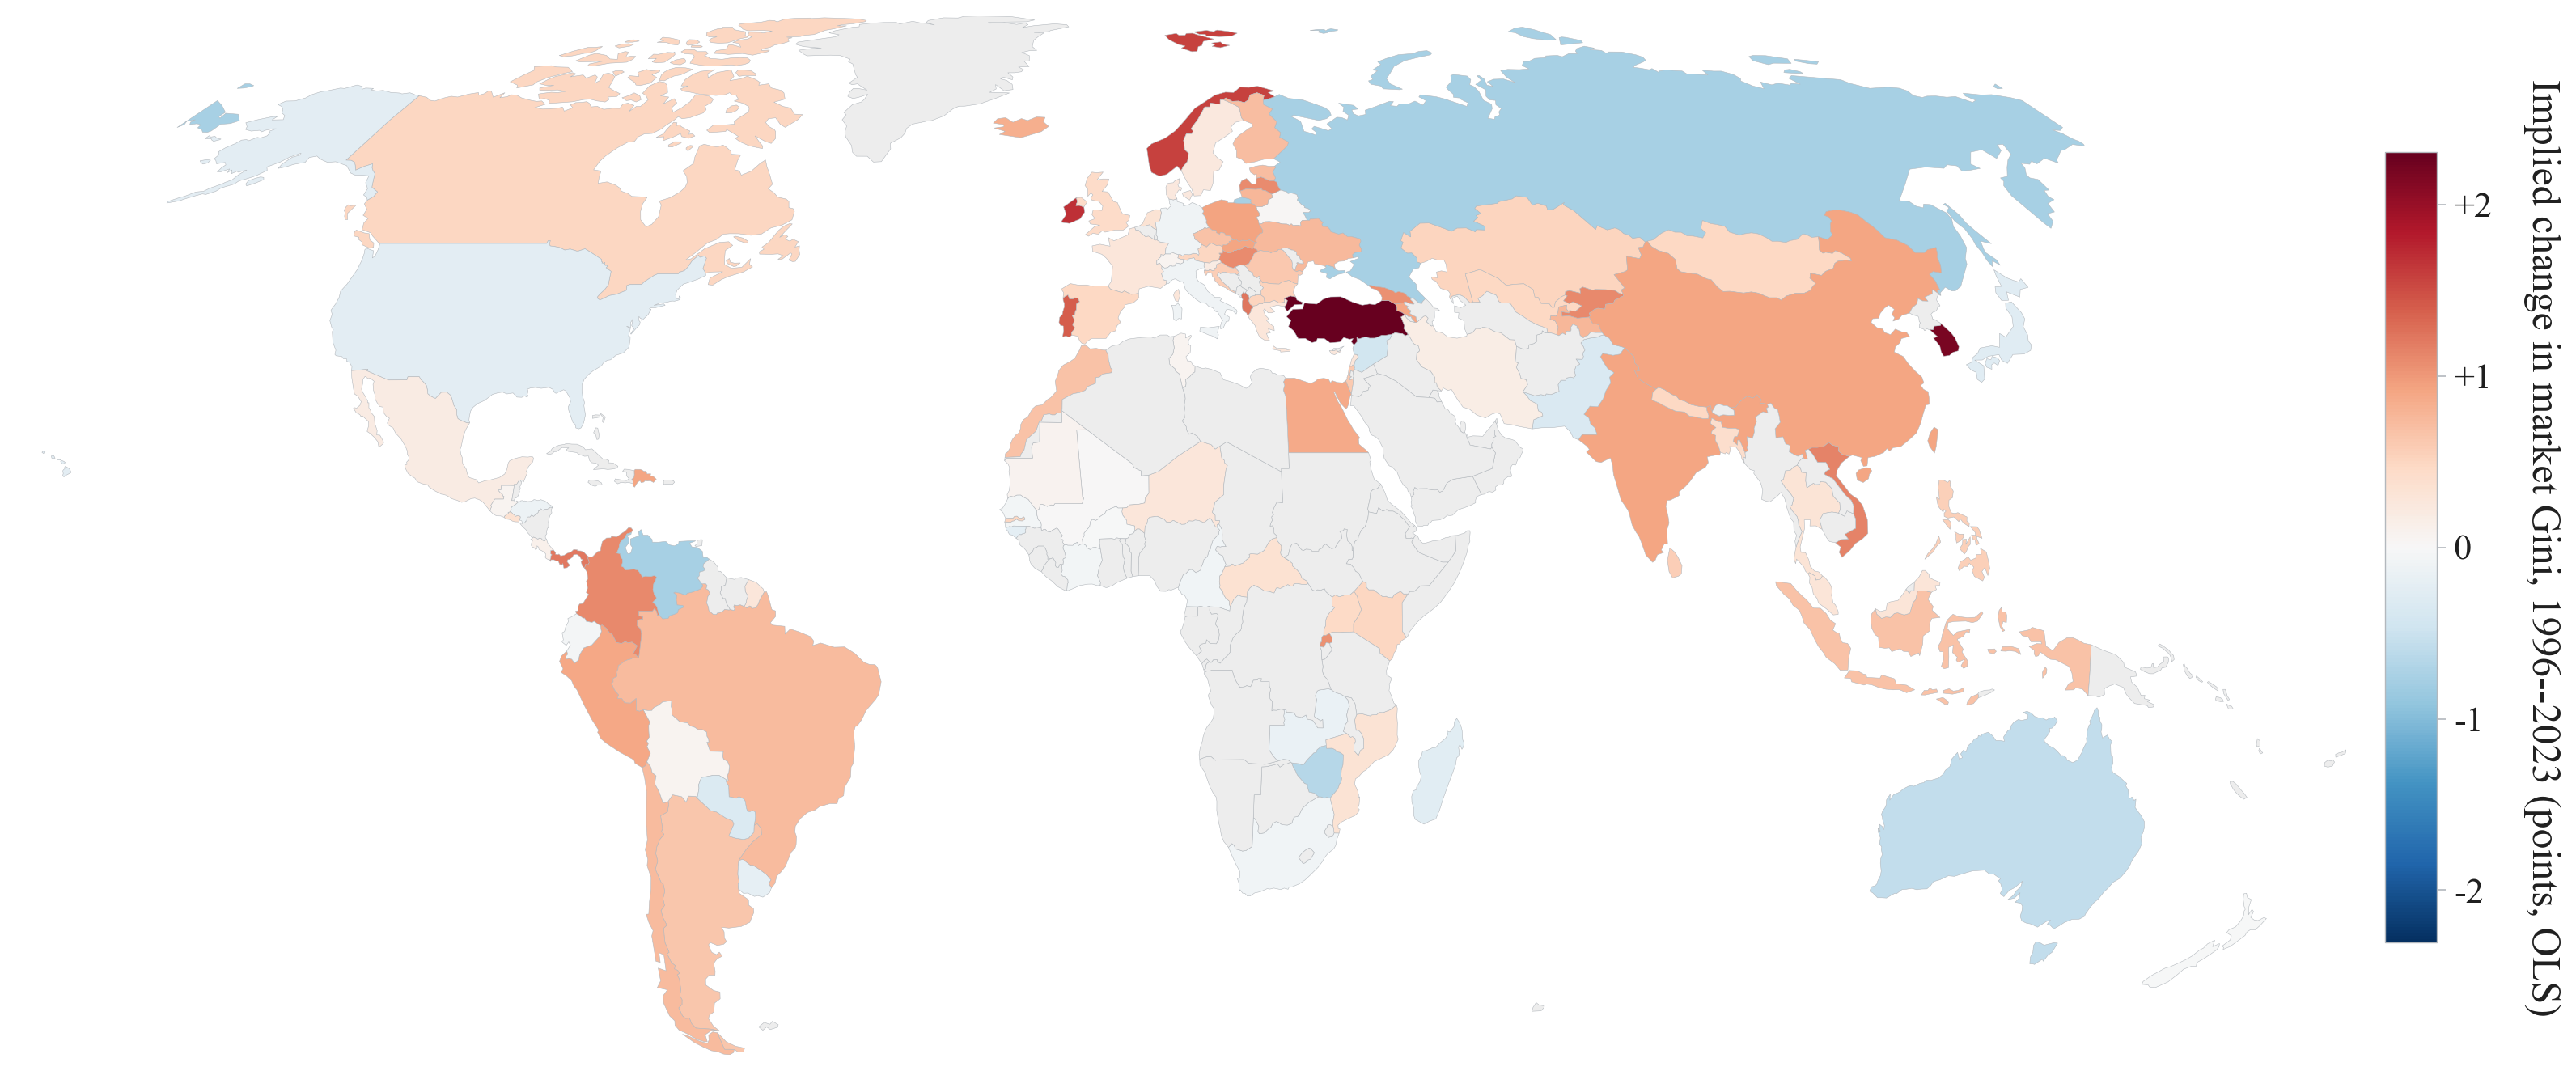
\includegraphics[width=\linewidth]{fig_map_implied_gini.png}
\caption{Implied change in the market Gini from hub-connectivity growth, 1996--2023, in points. The OLS coefficient ($0.061$) is applied to each country's change in $\ln\mathrm{GACI}_{max}$ between its first and last observation. Grey denotes economies not observed in both 1996--1998 and 2019--2023.}\label{fig:map_implied}\end{figure}

\section{Identification diagnostics and robustness}
\label{sec:diag}
Because both instruments are shift-share interactions with a single global shifter, the credibility of the 2SLS estimates depends on baseline exposure being unrelated to differential inequality trends. We conduct three sets of checks to address the concerns that (i) the exposure variable proxies for continent-level or income-group-level inequality trends, (ii) the instruments identify the level of connectivity but not its change, and (iii) the estimate is sensitive to specification and sample.

\subsection{Exposure-trend diagnostics}
Table~\ref{tab:diag} tightens the fixed-effects structure in steps. First, because a continent-level inequality trend correlated with baseline air market access would violate the exclusion restriction, we add continent by year fixed effects; the market-Gini estimate is $0.48$ with either instrument. Second, because other baseline characteristics may carry their own trends, we add baseline income, inequality, land area, latitude and sea market access, each interacted with the aviation index; the estimate falls to $0.38$ (Feyrer) and $0.44$ (tourism) with year fixed effects and to $0.28$ and $0.23$ with continent by year fixed effects. Third, income tercile and inequality tercile by year fixed effects give $0.34$ and $0.40$. With all of these together the Feyrer estimate is $0.33$ ($p<0.01$) and the tourism estimate $0.21$ ($p=0.13$); both instruments jointly, with continent by year fixed effects and exposure controls, give $0.31$ ($p<0.01$) with a Hansen $J$ $p$-value of $0.95$. The OLS estimate with the full interacted fixed-effects structure is $0.025$ ($p<0.01$). The market-Gini result is therefore not an artefact of continent-level or income-group-level inequality trends, although its magnitude falls by about a third once other exposures are allowed their own trends.

The disposable-Gini result is less robust. It is $0.13$ and not significant with continent by year fixed effects under the Feyrer instrument, $0.05$ with exposure controls and continent by year effects, and $0.08$ in the full specification; the tourism instrument gives $0.34$ ($p=0.03$) in the full specification, and the two instruments are rejected jointly ($J$ $p=0.04$). We therefore treat the market-income result as the finding and the disposable-income result as suggestive.

The first stage differs in sign across continents. Baseline air market access predicts faster hub-connectivity growth in Africa (first-stage coefficient $0.37$) and slower growth in Asia, Europe and Latin America ($-0.23$, $-0.33$ and $-0.21$), a pattern consistent with convergence within the already-connected continents and catch-up in Africa. The pooled first stage is positive because it combines within-continent and between-continent variation, and the reduced form inherits the same sign pattern (Table~\ref{tab:a_rfcont}). Sign heterogeneity in the first stage implies that the pooled 2SLS estimate is not a convex average of continent-specific effects, which is a further reason to prefer the continent by year specification and to report the continent-specific estimates in Table~\ref{tab:hetero}.

Dropping one continent at a time under continent by year fixed effects leaves the market estimate between $0.27$ and $0.58$ and significant, except when Asia is dropped and the first stage becomes weak. Under year fixed effects only, dropping Latin America reverses the sign, because Latin America combines low baseline air market access with the largest inequality decline in the sample; the reversal disappears once continent by year effects are included ($0.58$, $p<0.01$).

\begin{table}[H]\centering\caption{Identification diagnostics for the shift-share instruments.}\label{tab:diag}
\begin{threeparttable}\small\begin{tabular}{lcccc}
\toprule
Specification & Instrument & $\ln G^{mkt}$ & $\ln G^{disp}$ & KP $F$ \\
\midrule
Continent $\times$ year FE & Feyrer & 0.483\sym{***} (0.142) & 0.126 (0.109) & 16.7 \\
 & Tourism & 0.476\sym{**} (0.206) & 0.337\sym{*} (0.177) & 8.6 \\
Continent $\times$ year FE, drop Latin America & Feyrer & 0.579\sym{***} (0.181) & 0.238\sym{*} (0.135) & 12.3 \\
 & Tourism & 0.787\sym{*} (0.467) & 0.636 (0.404) & 3.1 \\
+ baseline exposures $\times$ aviation index & Feyrer & 0.377\sym{***} (0.063) & 0.506\sym{***} (0.077) & 79.4 \\
 & Tourism & 0.443\sym{***} (0.132) & 0.580\sym{***} (0.153) & 19.7 \\
+ exposures $\times$ index, continent $\times$ year FE & Feyrer & 0.275\sym{***} (0.103) & 0.048 (0.102) & 22.5 \\
 & Tourism & 0.232 (0.171) & 0.424\sym{*} (0.224) & 6.8 \\
Income tercile and Gini tercile $\times$ year FE & Feyrer & 0.342\sym{***} (0.056) & 0.484\sym{***} (0.071) & 86.0 \\
 & Tourism & 0.403\sym{***} (0.150) & 0.327\sym{**} (0.141) & 12.5 \\
All of the above & Feyrer & 0.334\sym{***} (0.117) & 0.083 (0.111) & 17.5 \\
 & Tourism & 0.205 (0.135) & 0.344\sym{**} (0.162) & 10.7 \\
Exposures $\times$ index, continent $\times$ year FE & Both & 0.306\sym{***} (0.103) & 0.214\sym{**} (0.101) & 12.8 \\
\quad Hansen $J$ $p$-value & & 0.95 & 0.04 & \\
OLS with all interacted FE & -- & 0.025\sym{***} (0.008) & 0.010 (0.009) & \\
\addlinespace\multicolumn{5}{l}{\emph{First stage by continent (coefficient on instrument, KP $F$)}}\\
Africa & Feyrer / Tourism & 0.365\sym{***} [40.6] & -0.018 [1.0] & \\
Asia & Feyrer / Tourism & -0.234\sym{***} [27.2] & 0.069\sym{**} [4.3] & \\
Europe & Feyrer / Tourism & -0.332\sym{***} [43.5] & -0.024 [1.7] & \\
Latin America & Feyrer / Tourism & -0.208\sym{**} [5.5] & 0.067\sym{***} [20.1] & \\
Middle East & Feyrer / Tourism & -0.451 [1.1] & 0.033 [0.3] & \\
North America & Feyrer / Tourism & 0.165 [1.1] & 0.072\sym{***} [11.3] & \\
Oceania & Feyrer / Tourism & -0.006 [0.0] & 0.123\sym{***} [51.7] & \\
\bottomrule
\end{tabular}
\begin{tablenotes}\footnotesize\item Robust SE in parentheses. Exposures interacted with the aviation index $a_t$: baseline ln GDP per capita, baseline market Gini, ln land area, absolute latitude and ln sea market access. \sym{*}~$p<0.10$, \sym{**}~$p<0.05$, \sym{***}~$p<0.01$.\end{tablenotes}\end{threeparttable}\end{table}

\subsection{Horizon, long differences and liberalisation episodes}
\label{sec:horizon}
The panel estimates are contemporaneous, so we next ask whether they reflect the timing of a response or the persistence of the series. Table~\ref{tab:horizon} and Figure~\ref{fig:horizon} examine the horizon. The 2SLS coefficient on connectivity lagged one to ten years is stable between $0.40$ and $0.52$, and the coefficient on connectivity led one to five years is as large or larger. A joint specification with current and three-year-ahead connectivity is uninformative because the two instruments are nearly collinear; Table~\ref{tab:a_leads} reports the lead coefficients. The lead pattern is what a persistent regressor and a trending instrument produce, and it does not distinguish anticipation from persistence.

Long differences are the natural design for a slow-moving outcome, and they are where the instruments lose power. In cross-sections of changes over 1996--2019, 2000--2019, 2005--2019 and 2010--2019 with continent fixed effects, the OLS coefficient is positive and imprecise ($0.03$ to $0.07$ for the market Gini). The first stage of the differenced Feyrer instrument is weak in every window, as is that of the differenced tourism instrument; stacked five-year differences give an estimate of $0.06$ ($p=0.46$) with the tourism instrument. The instruments therefore predict the level of connectivity within countries, through the interaction of a trending shifter with fixed exposure, but not its medium-run change. The 2SLS evidence is evidence on within-country co-movement, not on the response to discrete connectivity shocks.

Bilateral liberalisation is the third design. We collected the year in which each of 139 Open Skies agreements with the United States was first applied and estimate staggered difference-in-differences and event-study specifications, excluding the thirteen economies treated before 1997 (Table~\ref{tab:openskies}). Open Skies application does not move the connectivity measures: the post-treatment coefficient on ln hub connectivity is $0.02$ ($p=0.15$) and the event-study coefficients rise slowly to $0.05$ ten years after application without becoming significant. The market Gini rises by $0.024$ log points after application, but the event study shows a monotone pre-trend from $-0.018$ six years before to $-0.008$ one year before, so the post-treatment coefficients continue a trend rather than break one. The Callaway--Sant'Anna estimator with not-yet-treated controls gives the same result: an average treatment effect of $0.025$ ($p=0.22$) on ln hub connectivity and $0.017$ ($p=0.07$) on the market Gini. The event-study coefficients are reported in Tables~\ref{tab:a_es_conn} and \ref{tab:a_es_ineq}. As an instrument, Open Skies is weak; used together with the Feyrer instrument in an over-identified specification it gives a market-Gini coefficient of $0.427$ (Table~\ref{tab:a_osfeyrer}). The liberalisation design therefore neither confirms nor overturns the panel result.

\begin{figure}[H]\centering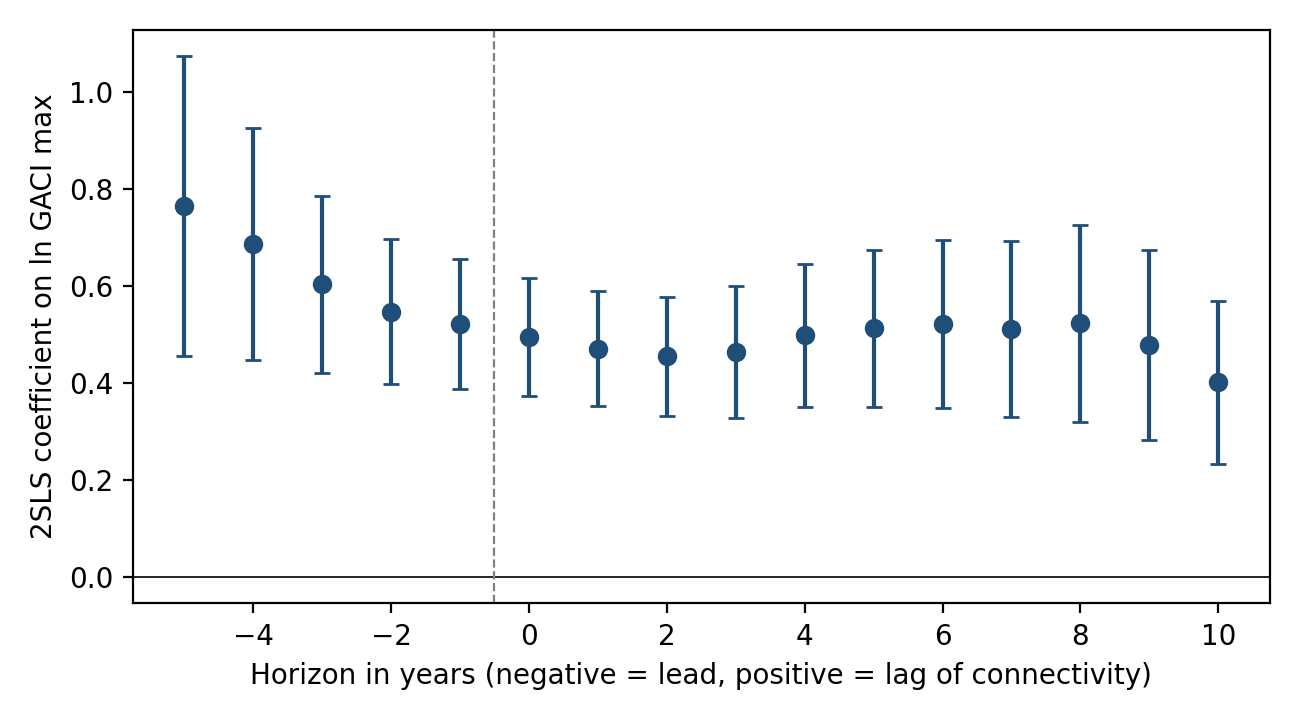
\includegraphics[width=0.75\textwidth]{fig_horizon.png}
\caption{2SLS coefficient on hub connectivity by horizon, market Gini, Feyrer instrument. Negative horizons are leads of connectivity; positive horizons are lags. Bars are 95 percent robust confidence intervals.}\label{fig:horizon}\end{figure}

\begin{table}[H]\centering\caption{Timing: lagged connectivity, long differences and stacked differences.}\label{tab:horizon}
\begin{threeparttable}\small\begin{tabular}{lcccc}
\toprule
Specification & $\ln G^{mkt}$ & $\ln G^{disp}$ & KP $F$ & N \\
\midrule
\multicolumn{5}{l}{\emph{Panel A. Lagged connectivity, 2SLS (instrument lagged equally)}}\\
Lag 0 & 0.495\sym{***} (0.062) & 0.651\sym{***} (0.077) & 98.5 & 3,735 \\
Lag 1 & 0.471\sym{***} (0.061) & 0.623\sym{***} (0.075) & 94.0 & 3,568 \\
Lag 2 & 0.455\sym{***} (0.063) & 0.617\sym{***} (0.078) & 86.0 & 3,401 \\
Lag 3 & 0.464\sym{***} (0.070) & 0.645\sym{***} (0.088) & 76.4 & 3,236 \\
Lag 5 & 0.513\sym{***} (0.082) & 0.712\sym{***} (0.105) & 63.6 & 2,912 \\
Lag 7 & 0.511\sym{***} (0.092) & 0.721\sym{***} (0.122) & 47.2 & 2,604 \\
Lag 10 & 0.402\sym{***} (0.086) & 0.588\sym{***} (0.112) & 38.3 & 2,144 \\
\addlinespace\multicolumn{5}{l}{\emph{Panel B. Long differences, cross-section with continent FE}}\\
1996--2019, OLS & 0.066 (0.045) & 0.026 (0.040) &  & 102 \\
1996--2019, 2SLS Feyrer & 1.749 (3.929) & 0.984 (2.329) & 0.16 & 102 \\
1996--2019, 2SLS tourism & 39.210 (1566.961) & 21.475 (857.209) & 0.00 & 102 \\
2000--2019, OLS & 0.056 (0.043) & 0.018 (0.036) &  & 106 \\
2000--2019, 2SLS Feyrer & 0.836 (0.986) & 0.358 (0.653) & 0.63 & 106 \\
2000--2019, 2SLS tourism & 2.201 (4.801) & 1.278 (2.964) & 0.18 & 106 \\
2005--2019, OLS & 0.055 (0.039) & 0.003 (0.039) &  & 114 \\
2005--2019, 2SLS Feyrer & 0.421 (0.370) & 0.074 (0.329) & 2.05 & 114 \\
2005--2019, 2SLS tourism & 0.647 (0.436) & 0.346 (0.337) & 2.91 & 114 \\
2010--2019, OLS & -0.043 (0.041) & -0.084\sym{*} (0.047) &  & 120 \\
2010--2019, 2SLS Feyrer & 1.921 (11.829) & 2.525 (15.596) & 0.03 & 120 \\
2010--2019, 2SLS tourism & 1.898 (3.340) & 0.643 (1.480) & 0.35 & 120 \\
Stacked 5-year differences, OLS & -0.007 (0.011) & -0.020 (0.014) &  & 2,914 \\
Stacked 5-year differences, 2SLS tourism & 0.063 (0.086) & 0.066 (0.089) & 12.79 & 2,914 \\
\bottomrule
\end{tabular}
\begin{tablenotes}\footnotesize\item Panel A: country and year fixed effects, robust SE. Panel B: cross-sections of changes with continent fixed effects, robust SE; stacked five-year differences with year and continent effects and country-clustered SE. \sym{*}~$p<0.10$, \sym{**}~$p<0.05$, \sym{***}~$p<0.01$.\end{tablenotes}\end{threeparttable}\end{table}

\begin{table}[H]\centering\caption{Open Skies agreements: staggered difference-in-differences and instrument.}\label{tab:openskies}
\begin{threeparttable}\small\begin{tabular}{lcccc}
\toprule
Outcome & DiD, country and year FE & DiD, continent $\times$ year FE & Pre-trend joint $F$ ($p$) & N \\
\midrule
ln GACI max & 0.020 (0.014) & 0.008 (0.012) & 1.56 (0.17) & 3,389 \\
ln GACI cwm & 0.017 (0.012) & 0.005 (0.010) & 1.69 (0.14) & 3,389 \\
ln GACI sum & 0.039 (0.042) & 0.016 (0.041) & 1.05 (0.39) & 3,389 \\
ln Gini, market & 0.024\sym{***} (0.007) & 0.014\sym{**} (0.006) & 2.90 (0.02) & 3,389 \\
ln Gini, disposable & 0.024\sym{***} (0.008) & 0.016\sym{**} (0.007) & 3.04 (0.01) & 3,389 \\
ln bottom 50\% share & -0.007 (0.018) & -0.005 (0.018) & 0.93 (0.46) & 3,368 \\
ln top 10\% share & 0.003 (0.010) & 0.005 (0.010) & 3.07 (0.01) & 3,368 \\
\addlinespace\multicolumn{5}{l}{\emph{Open Skies as instrument for ln GACI max (2SLS, clustered SE)}}\\
ln Gini, market & 1.195 (0.805) [KP $F$ 2.1] & 1.773 (2.739) & & 3,389 \\
ln Gini, disposable & 1.176 (0.796) [KP $F$ 2.1] & 2.066 (3.157) & & 3,389 \\
ln bottom 50\% share & -0.315 (0.859) [KP $F$ 2.2] & -0.682 (2.438) & & 3,368 \\
ln top 10\% share & 0.159 (0.484) [KP $F$ 2.2] & 0.635 (1.581) & & 3,368 \\
\bottomrule
\end{tabular}
\begin{tablenotes}\footnotesize\item Treatment is the year an Open Skies agreement with the United States was first applied; economies treated before 1997 are excluded. Country-clustered SE. Pre-trend $F$ tests the joint significance of event-time coefficients $-6$ to $-2$. \sym{*}~$p<0.10$, \sym{**}~$p<0.05$, \sym{***}~$p<0.01$.\end{tablenotes}\end{threeparttable}\end{table}

\subsection{Robustness}
Table~\ref{tab:robust} reports the remaining checks. First, because the baseline controls only for population, we add GDP per capita, urbanisation, tertiary enrolment, trade, tax revenue or sea market access; the market estimate remains between $0.49$ and $0.81$, and the increase with GDP per capita is the suppression documented in Table~\ref{tab:mech}. Second, because inference with seven continent clusters is imprecise, we compare clustering schemes; two-way clustering by continent and year widens the confidence interval to include zero, whereas Driscoll--Kraay errors give $p<0.01$. Third, because the leading hubs and the crisis years may drive the estimate, we drop the ten leading hub economies ($0.57$), restrict the sample to 1996--2019 ($0.44$) and drop 2008--09 and 2020--21 ($0.48$); the estimate is robust. Fourth, country-specific linear trends remove the identifying variation of an instrument that is nearly linear in time and give an uninformative estimate. Fifth, the survey-based World Bank Gini and decile shares, available for 1,877 country-years, give the same signs in both OLS and 2SLS: the Gini and the top-decile share rise and the bottom-quintile share falls.

Figure~\ref{fig:rfq} shows the reduced form by quintile of baseline inequality and baseline income. The reduced-form coefficient of the Feyrer instrument on the market Gini is positive in every income quintile except the richest, where it is zero, and positive in the second, fourth and fifth baseline-inequality quintiles. The association is therefore not driven by the richest or by the most unequal economies.

\begin{table}[H]\centering\caption{Robustness of the hub-connectivity estimate (2SLS, Feyrer instrument).}\label{tab:robust}
\begin{threeparttable}\small\begin{tabular}{lcccc}
\toprule
Specification & $\ln G^{mkt}$ & $\ln G^{disp}$ & KP $F$ / Hansen $p$ & N \\
\midrule
Baseline (ln population) & 0.495\sym{***} (0.062) & 0.651\sym{***} (0.077) & 98.5 & 3,735 \\
+ ln GDP per capita & 0.753\sym{***} (0.109) & 0.968\sym{***} (0.140) & 55.9 & 3,735 \\
+ urban share & 0.504\sym{***} (0.063) & 0.663\sym{***} (0.078) & 98.1 & 3,735 \\
+ tertiary enrolment & 0.546\sym{***} (0.137) & 0.757\sym{***} (0.169) & 26.0 & 2,508 \\
+ trade/GDP & 0.486\sym{***} (0.062) & 0.651\sym{***} (0.078) & 92.5 & 3,725 \\
+ tax/GDP & 0.667\sym{***} (0.160) & 0.899\sym{***} (0.196) & 28.5 & 2,595 \\
+ ln sea market access & 0.535\sym{***} (0.071) & 0.718\sym{***} (0.089) & 88.6 & 3,735 \\
+ GDP pc, urban, tertiary, trade & 0.814\sym{***} (0.263) & 1.118\sym{***} (0.337) & 12.4 & 2,500 \\
Both instruments (Hansen $J$ $p$ in col. 4) & 0.490\sym{***} (0.055) & 0.606\sym{***} (0.064) & 67.5 / 0.88 & 3,735 \\
Tourism instrument only & 0.468\sym{***} (0.165) & 0.391\sym{***} (0.151) & 13.6 & 3,735 \\
SE clustered by country & 0.495\sym{**} (0.194) & 0.651\sym{***} (0.241) & 10.6 & 3,735 \\
SE two-way clustered continent, year & 0.495 (0.424) & 0.651 (0.471) & 15.6 & 3,735 \\
Driscoll--Kraay SE (3 lags) & 0.495\sym{***} (0.069) & 0.651\sym{***} (0.096) & 20.2 & 3,735 \\
Drop ten leading hub economies & 0.565\sym{***} (0.066) & 0.709\sym{***} (0.082) & 94.0 & 3,472 \\
1996--2019 only & 0.439\sym{***} (0.052) & 0.574\sym{***} (0.064) & 118.6 & 3,344 \\
Drop 2008--09 and 2020--21 & 0.480\sym{***} (0.056) & 0.635\sym{***} (0.071) & 114.9 & 3,204 \\
Continent $\times$ year FE & 0.483\sym{***} (0.142) & 0.126 (0.109) & 16.7 & 3,734 \\
Country-specific linear trends & -0.740 (0.652) & -0.808 (0.740) & 1.3 & 3,735 \\
\addlinespace\multicolumn{5}{l}{\emph{Leave-one-continent-out (country and year FE)}}\\
Drop Africa & 0.683\sym{***} (0.094) & 0.885\sym{***} (0.120) & 63.9 & 2,790 \\
Drop Asia & 0.712\sym{***} (0.092) & 0.824\sym{***} (0.107) & 76.2 & 3,110 \\
Drop Europe & 0.313\sym{***} (0.057) & 0.504\sym{***} (0.078) & 56.6 & 2,604 \\
Drop Latin America & -0.080\sym{**} (0.041) & 0.010 (0.037) & 78.6 & 3,179 \\
Drop Middle East & 0.603\sym{***} (0.080) & 0.787\sym{***} (0.101) & 80.5 & 3,498 \\
Drop North America & 0.568\sym{***} (0.069) & 0.733\sym{***} (0.087) & 88.0 & 3,658 \\
Drop Oceania & 0.576\sym{***} (0.076) & 0.774\sym{***} (0.097) & 80.2 & 3,571 \\
\bottomrule
\end{tabular}
\begin{tablenotes}\footnotesize\item Robust SE in parentheses unless the row states otherwise. \sym{*}~$p<0.10$, \sym{**}~$p<0.05$, \sym{***}~$p<0.01$.\end{tablenotes}\end{threeparttable}\end{table}

\begin{figure}[H]\centering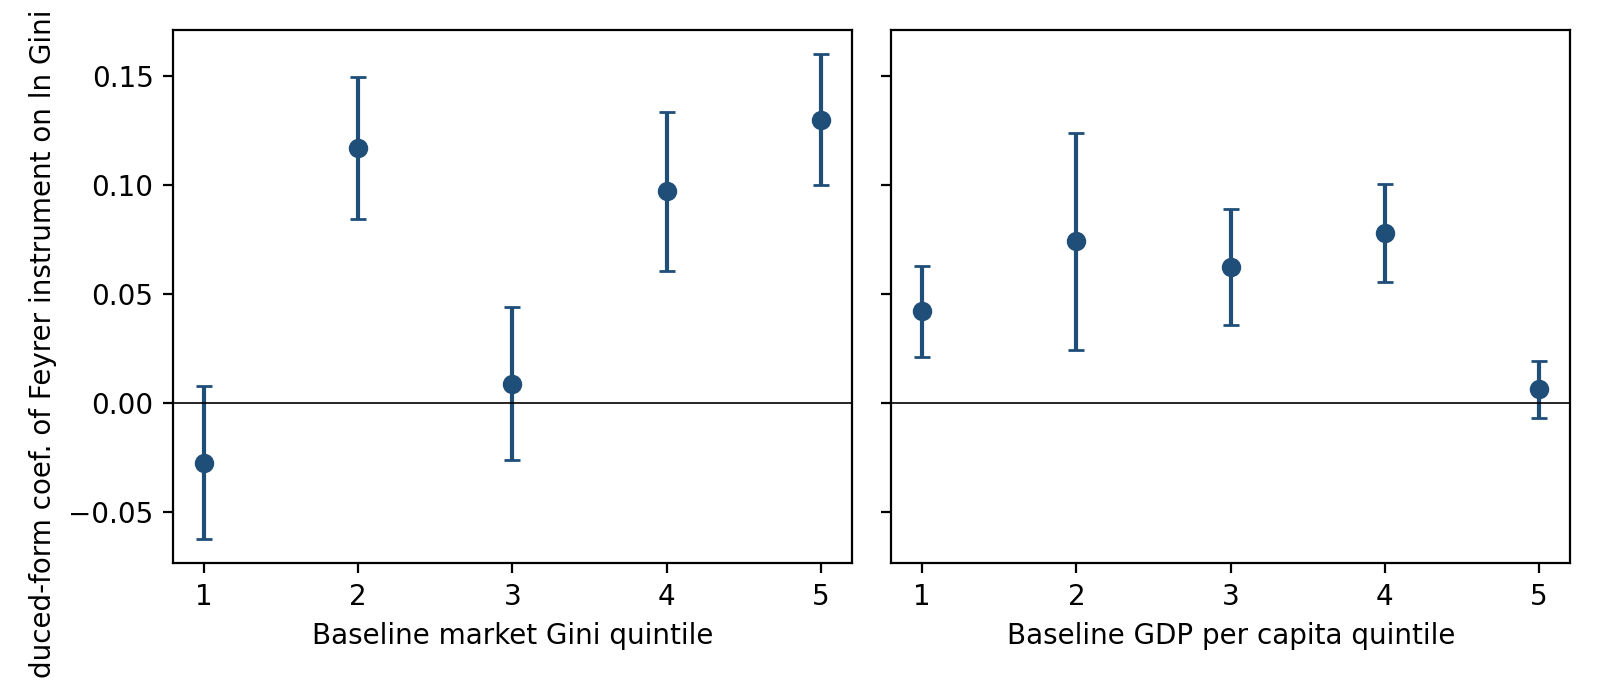
\includegraphics[width=0.85\textwidth]{fig_rf_quintile.png}
\caption{Reduced-form coefficient of the Feyrer instrument on the market Gini by quintile of baseline inequality (left) and baseline income (right). Country and year fixed effects; 95 percent robust confidence intervals.}\label{fig:rfq}\end{figure}

\section{Synthesis: the hypotheses revisited}
\label{sec:synthesis}
First, Hypothesis~1 is supported for market inequality and not for attenuation by redistribution. Within countries, rising hub connectivity accompanies a rising market Gini in OLS, in 2SLS with two different instruments, and under continent by year and income-group by year fixed effects. The disposable Gini rises by at least as much, and the redistribution wedge narrows.

Second, Hypothesis~2 is supported at the bottom half and the top decile and rejected at the top percentile. The pretax income share of the bottom half falls, the top decile share rises by less, and the top percentile share does not move. The distributional response to connectivity is a widening between the upper-middle of the distribution and the bottom half rather than an increase at the very top. Measured in levels, the same result is an average income gain of which the bottom half retains about one third, and the ratio of top-decile to bottom-half average income is the one growth quantity that survives the continent by year and over-identification checks.

Third, Hypothesis~3 is supported. At a given total connectivity, a network concentrated in one gateway is associated with higher inequality and dispersion across airports with lower inequality, and the marginal gateway gain is associated with the largest increase in inequality where the network was previously distributed.

Fourth, Hypothesis~4 is supported. Connectivity raises income, industrial employment and urbanisation, each of which is associated with lower inequality, so the residual association is larger than the total; unemployment is the only channel that operates in the same direction.

Two qualifications bound these conclusions. First, the 2SLS magnitudes are too large to be structural elasticities, as the aggregate contribution exercise shows, and the relevant order of magnitude is the OLS one: about half a Gini point for the average country's connectivity growth since 1996. Second, neither long differences nor liberalisation episodes move connectivity with sufficient precision, so the evidence is on co-movement within countries rather than on the response to identified shocks.

\section{Conclusion}
\label{sec:conclusion}
Gateway connectivity is associated with growth, and this paper asks who receives it. Using a global panel of 166 economies over 1996--2023, we find that within-country increases in the connectivity of the primary hub accompany increases in market-income inequality, located in a falling income share of the bottom half and a rising share of the top decile, with no response at the top percentile. The association is present under continent by year and income-group by year fixed effects, is larger in Asia and after 2010, is reversed in Africa, and is larger in networks where connectivity is concentrated in a single gateway at a given total. It is not a by-product of growth: the income, industrial employment and urbanisation that connectivity induces are associated with lower inequality, and the residual association is larger than the total.

The policy reading follows the companion paper's distinction between hub concentration and distributed access. If the objective is the aggregate, the gateway is where the return to connectivity is largest; if the objective includes the distribution, the same connectivity spread across secondary airports is associated with a smaller increase in inequality. The evidence is on co-movement rather than on shock responses, and the next step is subnational: airport-level connectivity matched to local income and night-light data would identify whether the gateway region's gain is offset elsewhere in the country, which is the mechanism that this paper's national estimates imply but cannot observe.

\bibliographystyle{elsarticle-harv}
\bibliography{refs_inequality}
\end{document}
